\documentclass[english,a4paper,12pt]{report}
\usepackage{fancyhdr}
\usepackage{comment}
\usepackage{iftex}
\usepackage{graphicx}
\usepackage{geometry}
\usepackage{booktabs}
\usepackage{enumerate}
\usepackage{tabularx}
\usepackage{amsfonts}
\usepackage{blindtext}
\usepackage{qtree}
\usepackage{multicol}
\usepackage{amsmath,bm}
\usepackage{float}
\usepackage{amssymb}
\usepackage{wrapfig}
\restylefloat{figure}
\newcommand{\tabitem}{~~\llap{\textbullet}~~}
\usepackage{minted}
\usepackage{listings}
% \lstset{
%  basicstyle=\footnotesize,
%  language={[Objective]Caml},
%  breaklines=true,
%  tabsize=2,
%  frame=single,
%  numbers=left,
%  title=\lstname,
%  commentstyle=\color{mygreen},
%  numberstyle=\small\color{mygray},
%  stringstyle=\color{mymauve},
%  showstringspaces=false,
%  rulecolor=\color{black}
% }

\usepackage{xcolor}
\definecolor{codegreen}{rgb}{0,0.6,0}
\definecolor{codegray}{rgb}{0.5,0.5,0.5}
\definecolor{codepurple}{rgb}{0.58,0,0.82}
\definecolor{backcolour}{rgb}{0.95,0.95,0.92}
%Code listing style named "mystyle"

\usepackage{color}
\usepackage[draft=false]{hyperref}
\hypersetup{
    colorlinks=true, % make the links colored
    linkcolor=blue, % color TOC links in blue
    urlcolor=blue, % color URLs in blue
    linktoc=all % 'all' will create links for everything in the TOC
}
    
\urlstyle{same}
\lstdefinestyle{mystyle}{
  backgroundcolor=\color{backcolour},   commentstyle=\color{codegreen},
  keywordstyle=\color{magenta},
  numberstyle=\tiny\color{codegray},
  stringstyle=\color{codepurple},
  basicstyle=\ttfamily\footnotesize,
  breakatwhitespace=false,         
  breaklines=true,                 
  captionpos=b,     
  upquote=true,
  keepspaces=true,                 
  numbers=left,                    
  numbersep=5pt,                  
  showspaces=false,                
  showstringspaces=false,
  showtabs=false,                  
  tabsize=2
}


%"mystyle" code listing set
\lstset{style=mystyle}
\geometry{verbose,tmargin=4.5cm,bmargin=4cm,lmargin=1.5cm,rmargin=1cm,headheight=2.7cm,headsep=1.5cm,footskip=2cm}
\usepackage{array}
%
\def \hsp {\hspace{3mm}}
%
\makeatletter
\providecommand{\tabularnewline}{\\}
\makeatother
%
\ifxetex
\usepackage[T1]{fontenc}
\usepackage{fontspec}
\newfontfamily\nakulafont[AutoFakeBold=2]{Nakula}
\newfontfamily\liberationfont{Liberation Sans Narrow}
\newfontfamily\liberationsansfont{Liberation Sans}
\fi
%
\usepackage{tikz}
\usepackage{xcolor}
%
% 
\definecolor{circleorange}{rgb}{1,0.17,0.08}
\definecolor{darkorange}{rgb}{1,0.27,0.1}
\definecolor{orange2}{rgb}{1,0.5,0.15}
\definecolor{orange3}{rgb}{1,0.65,0.25}
\definecolor{yellow1}{rgb}{0.95,0.77,0.2}
\newcommand{\Omit}[1]{}
\fancypagestyle{plain}{
  \fancyhead[LO]
  {
\textbf{CS4443 - Software Engineering} \newline 
\textbf {Indian Institute of Technology Hyderabad \newline
System Requirement Analysis\newline 
Group: H16} \newline 
	  }
	  
%
	  \fancyhf[ROH]{

\begin{tikzpicture}[scale=0.25,every node/.style={transform shape}]
\draw [fill=circleorange,circleorange] (5,10) circle (1.15); 
\fill [darkorange] (5.06,8) -- (5.06,2) -- (7.3,1.2) -- (7.3,8.8) -- (5.06,8);
\fill [darkorange] (4.94,8) -- (4.94,2) -- (2.7,1.2) -- (2.7,8.8) -- (4.94,8);
\fill [orange2]    (7.4,8.4) -- (7.4,1.6) -- (8.2,1.2) -- (8.2,8.8) -- (7.4,8.4);
\fill [orange2]    (2.6,8.4) -- (2.6,1.6) -- (1.8,1.2) -- (1.8,8.8) -- (2.6,8.4);
\fill [orange3]    (8.3,8.4) -- (8.3,1.6) -- (9.0,1.2) -- (9.0,8.8) -- (8.3,8.4);
\fill [orange3]    (1.7,8.4) -- (1.7,1.6) -- (1.0,1.2) -- (1.0,8.8) -- (1.7,8.4);
\fill [yellow1]    (9.1,8.4) -- (9.1,1.6) -- (9.7,1.2) -- (9.7,8.8) -- (9.1,8.4);
\fill [yellow1]    (0.9,8.4) -- (0.9,1.6) -- (0.3,1.2) -- (0.3,8.8) -- (0.9,8.4);
\ifxetex
\node [scale=2.1] at (5,-0.1)  {   {\bf {\nakulafont  भारतीय प्रौद्योगिकी संस्थान हैदराबाद }} };
\node [scale=1.8] at (5,-1.2) {   {\bf {\liberationsansfont Indian Institute of Technology Hyderabad}} };
\fi
\end{tikzpicture}
		  }
%
\renewcommand\headrule
 {

\begin{tikzpicture}
\definecolor{yellow1}{rgb}{0.95,0.77,0.2}
\draw[line width=0.75mm, yellow1] (0,0) -- (\textwidth,0);
\end{tikzpicture} 
 }}
 \pagestyle{plain}


\title{\textbf{\underline{\Huge{System Requirement Analysis}}}\\~\\
\textbf{Conference Management System}\\~\\ 
Professor Manish Singh\\
}
\author{Vinta Reethu \and Havya Sree K \and Dheekshitha B \and Akash Tadwai }
\date{\today}
\usepackage{titlesec}

\begin{document}
\titleformat{\chapter}[display]   
{\normalfont\huge\bfseries}{\chaptertitlename\ \thechapter}{20pt}{\Huge}   
\titlespacing*{\chapter}{0pt}{-10pt}{40pt}
\maketitle

\newpage

\section*{Context Diagram}
\addcontentsline{toc}{chapter}{Context Diagram}
\begin{figure}[h!]
\centering
 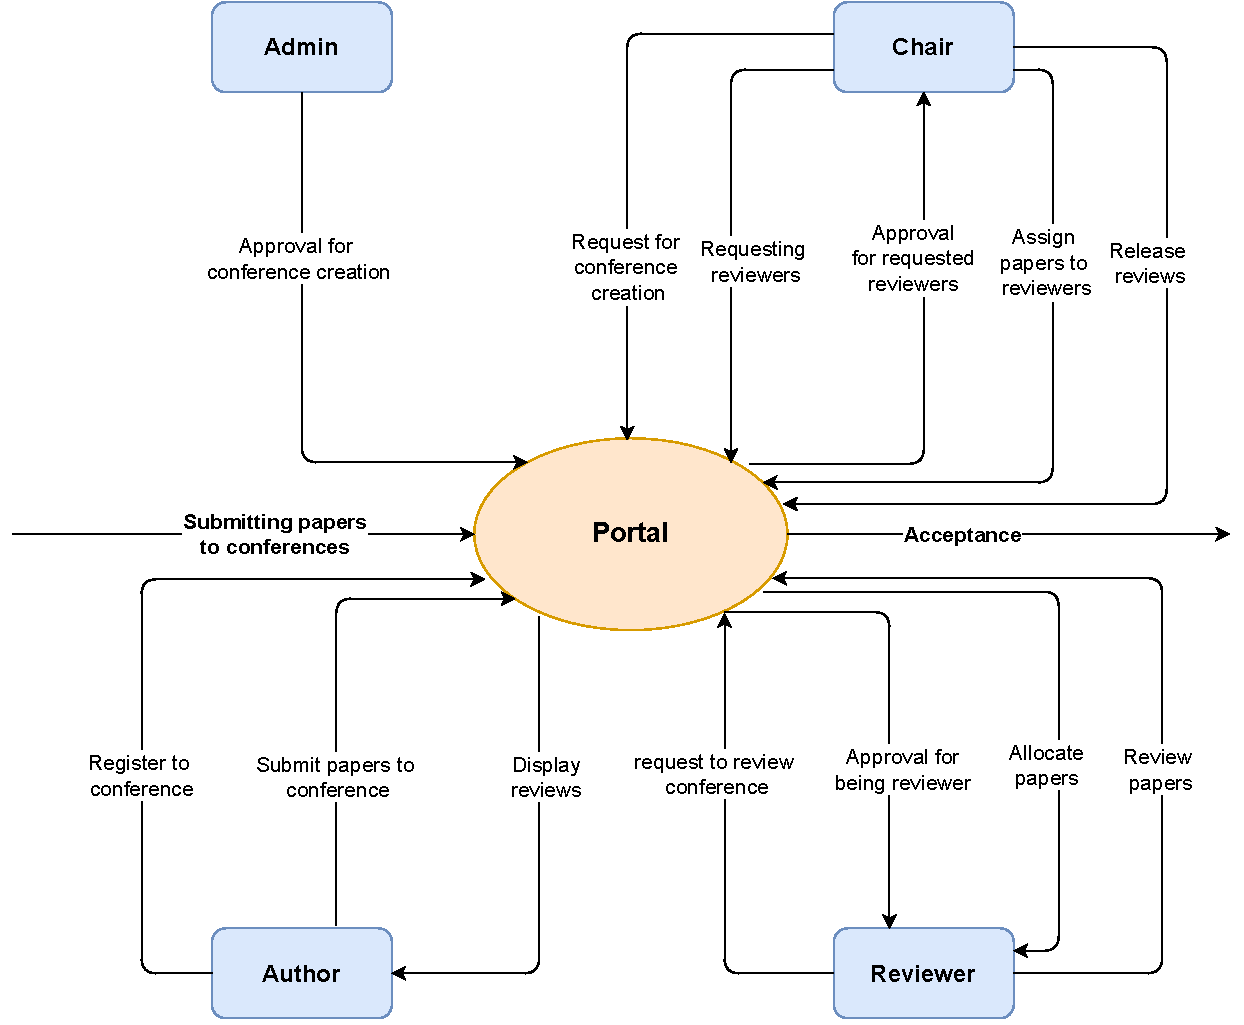
\includegraphics[keepaspectratio,width=17cm,height=12cm]{SRA-Images/context-diagram.pdf}
\caption{Context Diagram}
\end{figure}

Our conference system management will have 4 entities i.e Admin, Conference Chair, Reviewer, Author. 
\begin{enumerate}
    \item \textbf{Admin}: The admin is the person who installs, updates, and restores the system. He/she is also in charge of setting up an account for chairs if their conference request is accepted.
    \item \textbf{Conference Chair}: The person who makes the overall decisions like assigning papers to reviewers. 
    \item \textbf{Reviewer}: Reviewer is a member of the program committee assigned by the chair to review authors' submission.
    \item \textbf{Author}: The person who submits abstracts and full papers.
\end{enumerate}
\vspace{2cm}
\section*{Data Flow Diagrams}
\addcontentsline{toc}{chapter}{Data Flow Diagrams}
\hspace{1cm} \textbf{\textit{Data flow diagrams}} is a type of diagram that depicts the movement of data through a system or process and are crucial in the system or software design process. For our software, we decided to split into two teams, each with their own concept of what the product should be and the DFDs that go with it. We finally integrated the two DFDs into a new one, integrating the benefits of both and eliminating most of their shortcomings, after discussing, evaluating, and criticising each other's DFDs. This document seeks to offer some insight on the design process behind each DFD, as well as how we arrived at the final DFD and its key features.

\begin{enumerate}
    \item \textbf{DFD of First Team}
    \addcontentsline{toc}{section}{DFD-Team1}
    \begin{figure}[h!]
\centering
 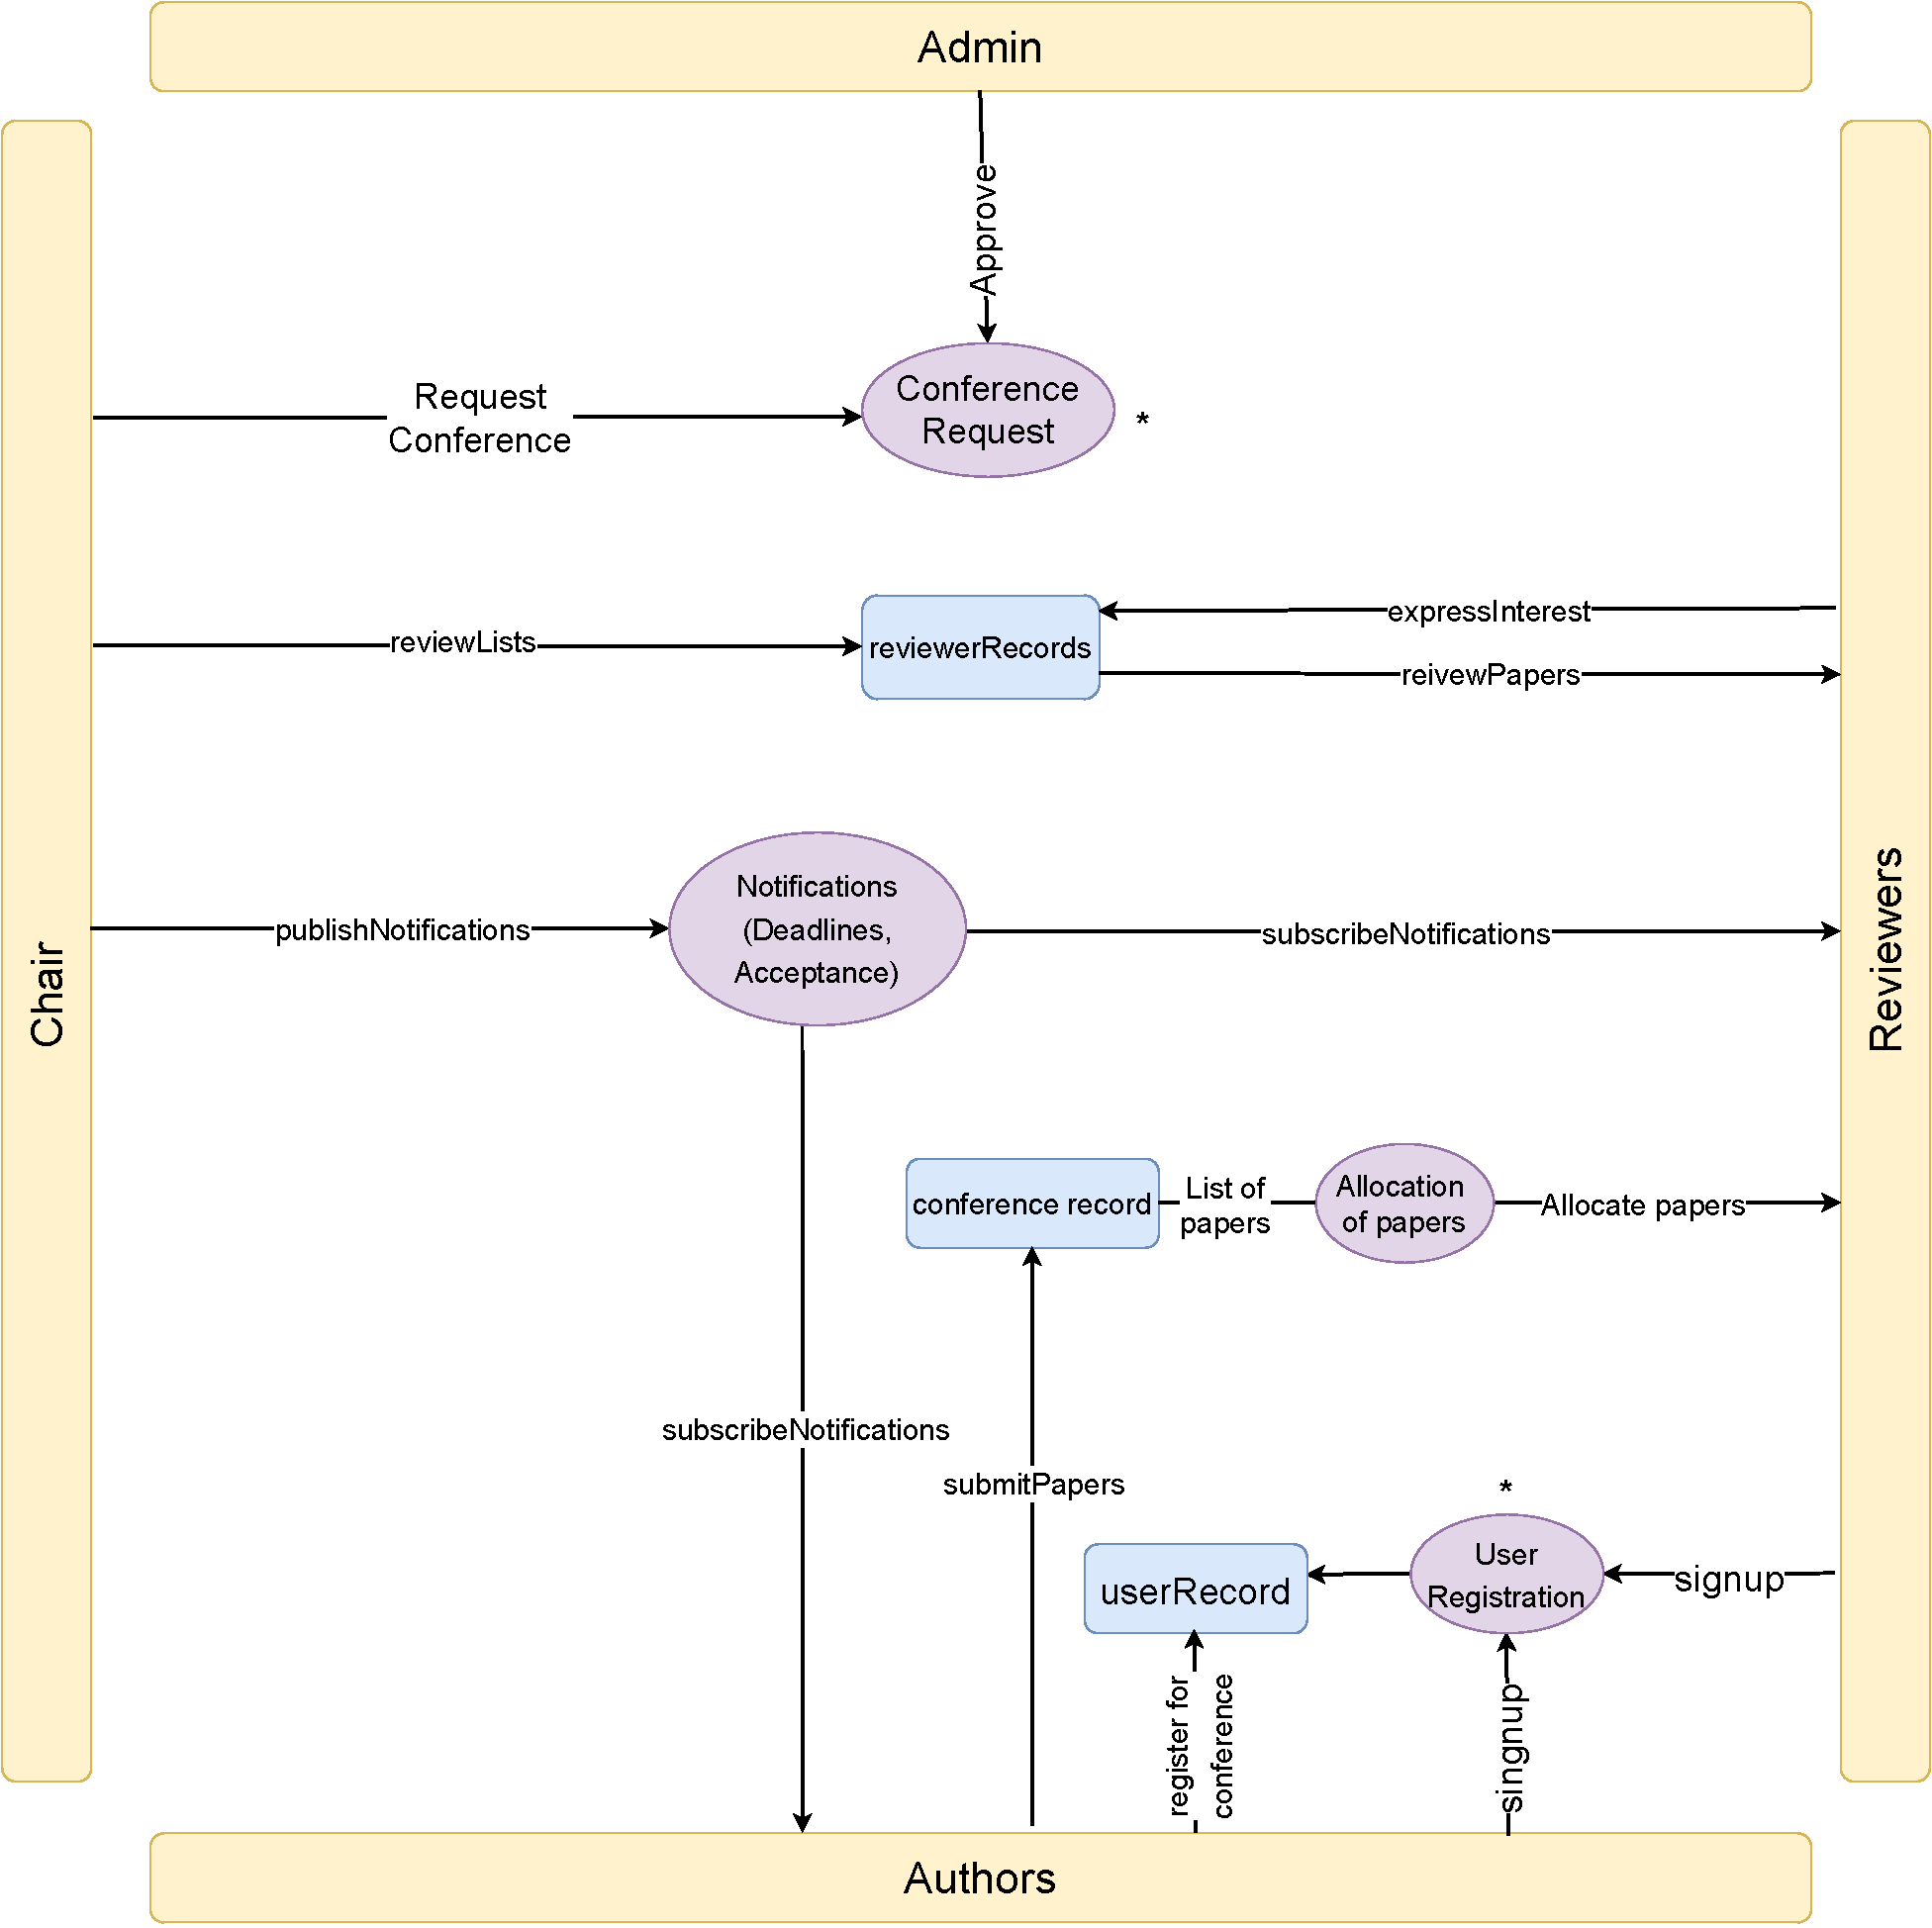
\includegraphics[keepaspectratio,width=25cm,height=12cm]{SRA-Images/DFD-Team1.pdf}
 \caption{Data Flow Diagram - Team 1}
\end{figure}

\begin{itemize}
    \item The principal entities are Admin, Conference Chair, Authors, Reviewers. 
    \item Conference chair requests for hosting a conference on the portal and Admin verifies the details of the conference and approves it.
    \item Users (Authors, Reviewers) get registered on the conference portal and these credentials are stored in \textit{User Records}
    \item Authors subscribe for the conferences for which they are willing to submit papers.
    \item Authors submit papers in their interested conferences and this data  is stored in \textit{conference record}.
    \item Before Authors can submit papers, the chair can either request reviewers or reviewers can express their interest to review at a particular conference. The final list of reviewers and their interests are stored in \textit{reviewerRecords}.
    \item All the Papers submitted before the deadline in a conference are allocated to Reviewers by the \textit{allocation algorithm} upon their interest such that for every paper there are atleast 3 reviewers.
    \item Chair sends different kinds of notifications for Reviewers \&  Authors regarding deadlines, Acceptance, Camera Ready submission etc. Users and Reviewers subscribe to the notifications sent by the author.
    \item DFD doesn't tackle how exactly the authentication mechanism for users work. It doesn't tackle how the reviews are being displayed to the user.
    \item DFD doesn't provide any clarity on how the paper allocation process works. It also doesn't give any information about which APIs are being used for notification service.
\end{itemize}

\item \textbf{DFD of Second Team}
\addcontentsline{toc}{section}{DFD-Team2}
\begin{figure}[h!]
 \centering
 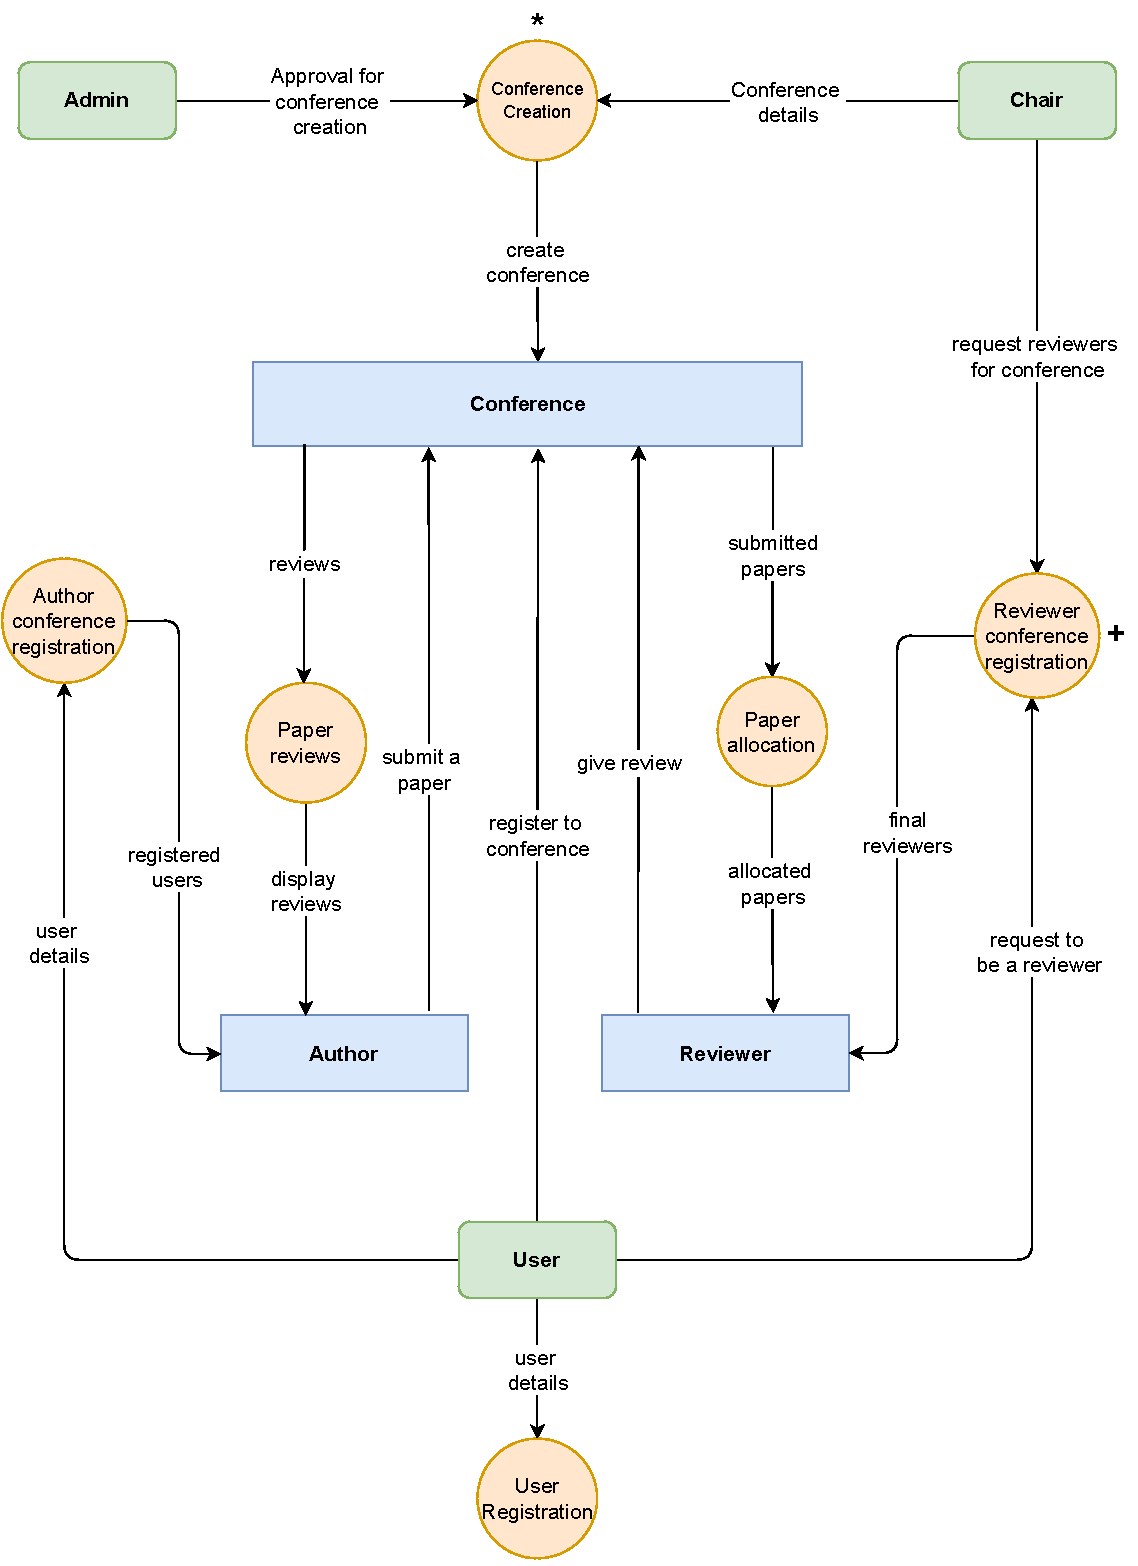
\includegraphics[keepaspectratio,height=15cm]{SRA-Images/DFD-team2.pdf}
 \caption{Data Flow Diagram - Team 2}
\end{figure}

\begin{itemize}
    \item The principal entities are Admin, Conference Chair, Users. 
    \item A user using the website for the first time should register his identity by providing his details. 
    \item A user should register to a conference to be an author or can also request the chair person to be a reviewer. He can also accept or reject a request from the chair person to be a reviewer of a conference.
    \item If the user is registered to a conference as an author, he can submit papers to the conference. An author can see the status of their paper and its reviews for his submitted papers after a deadline.
    \item If the user is permitted to be a reviewer, he gets papers allocated by the conference that he needs to review  before the deadline. 
    \item A chair person of the conference requests the Admin to host a conference by providing the conference details. 
    \item The chair person finalises set of reviewers for the conference by requesting users to be reviewers or by approving requests from users to be a reviewer based on their interests. After the paper submission deadline, the chair person also allocates atleast 3 reviewers to each paper.
    \item Admin maintains the conference portal and host approved conferences on the portal.
    \item The DFD does not give any information regarding how the chair person notifies the authors/reviewers(e.g.\ notifying author before paper deadline) and also it doesn't provide any clarity on how the paper allocation process works.
    
\end{itemize}
\item \textbf{Final DFD} \\
    \begin{figure}[h!]
\centering
 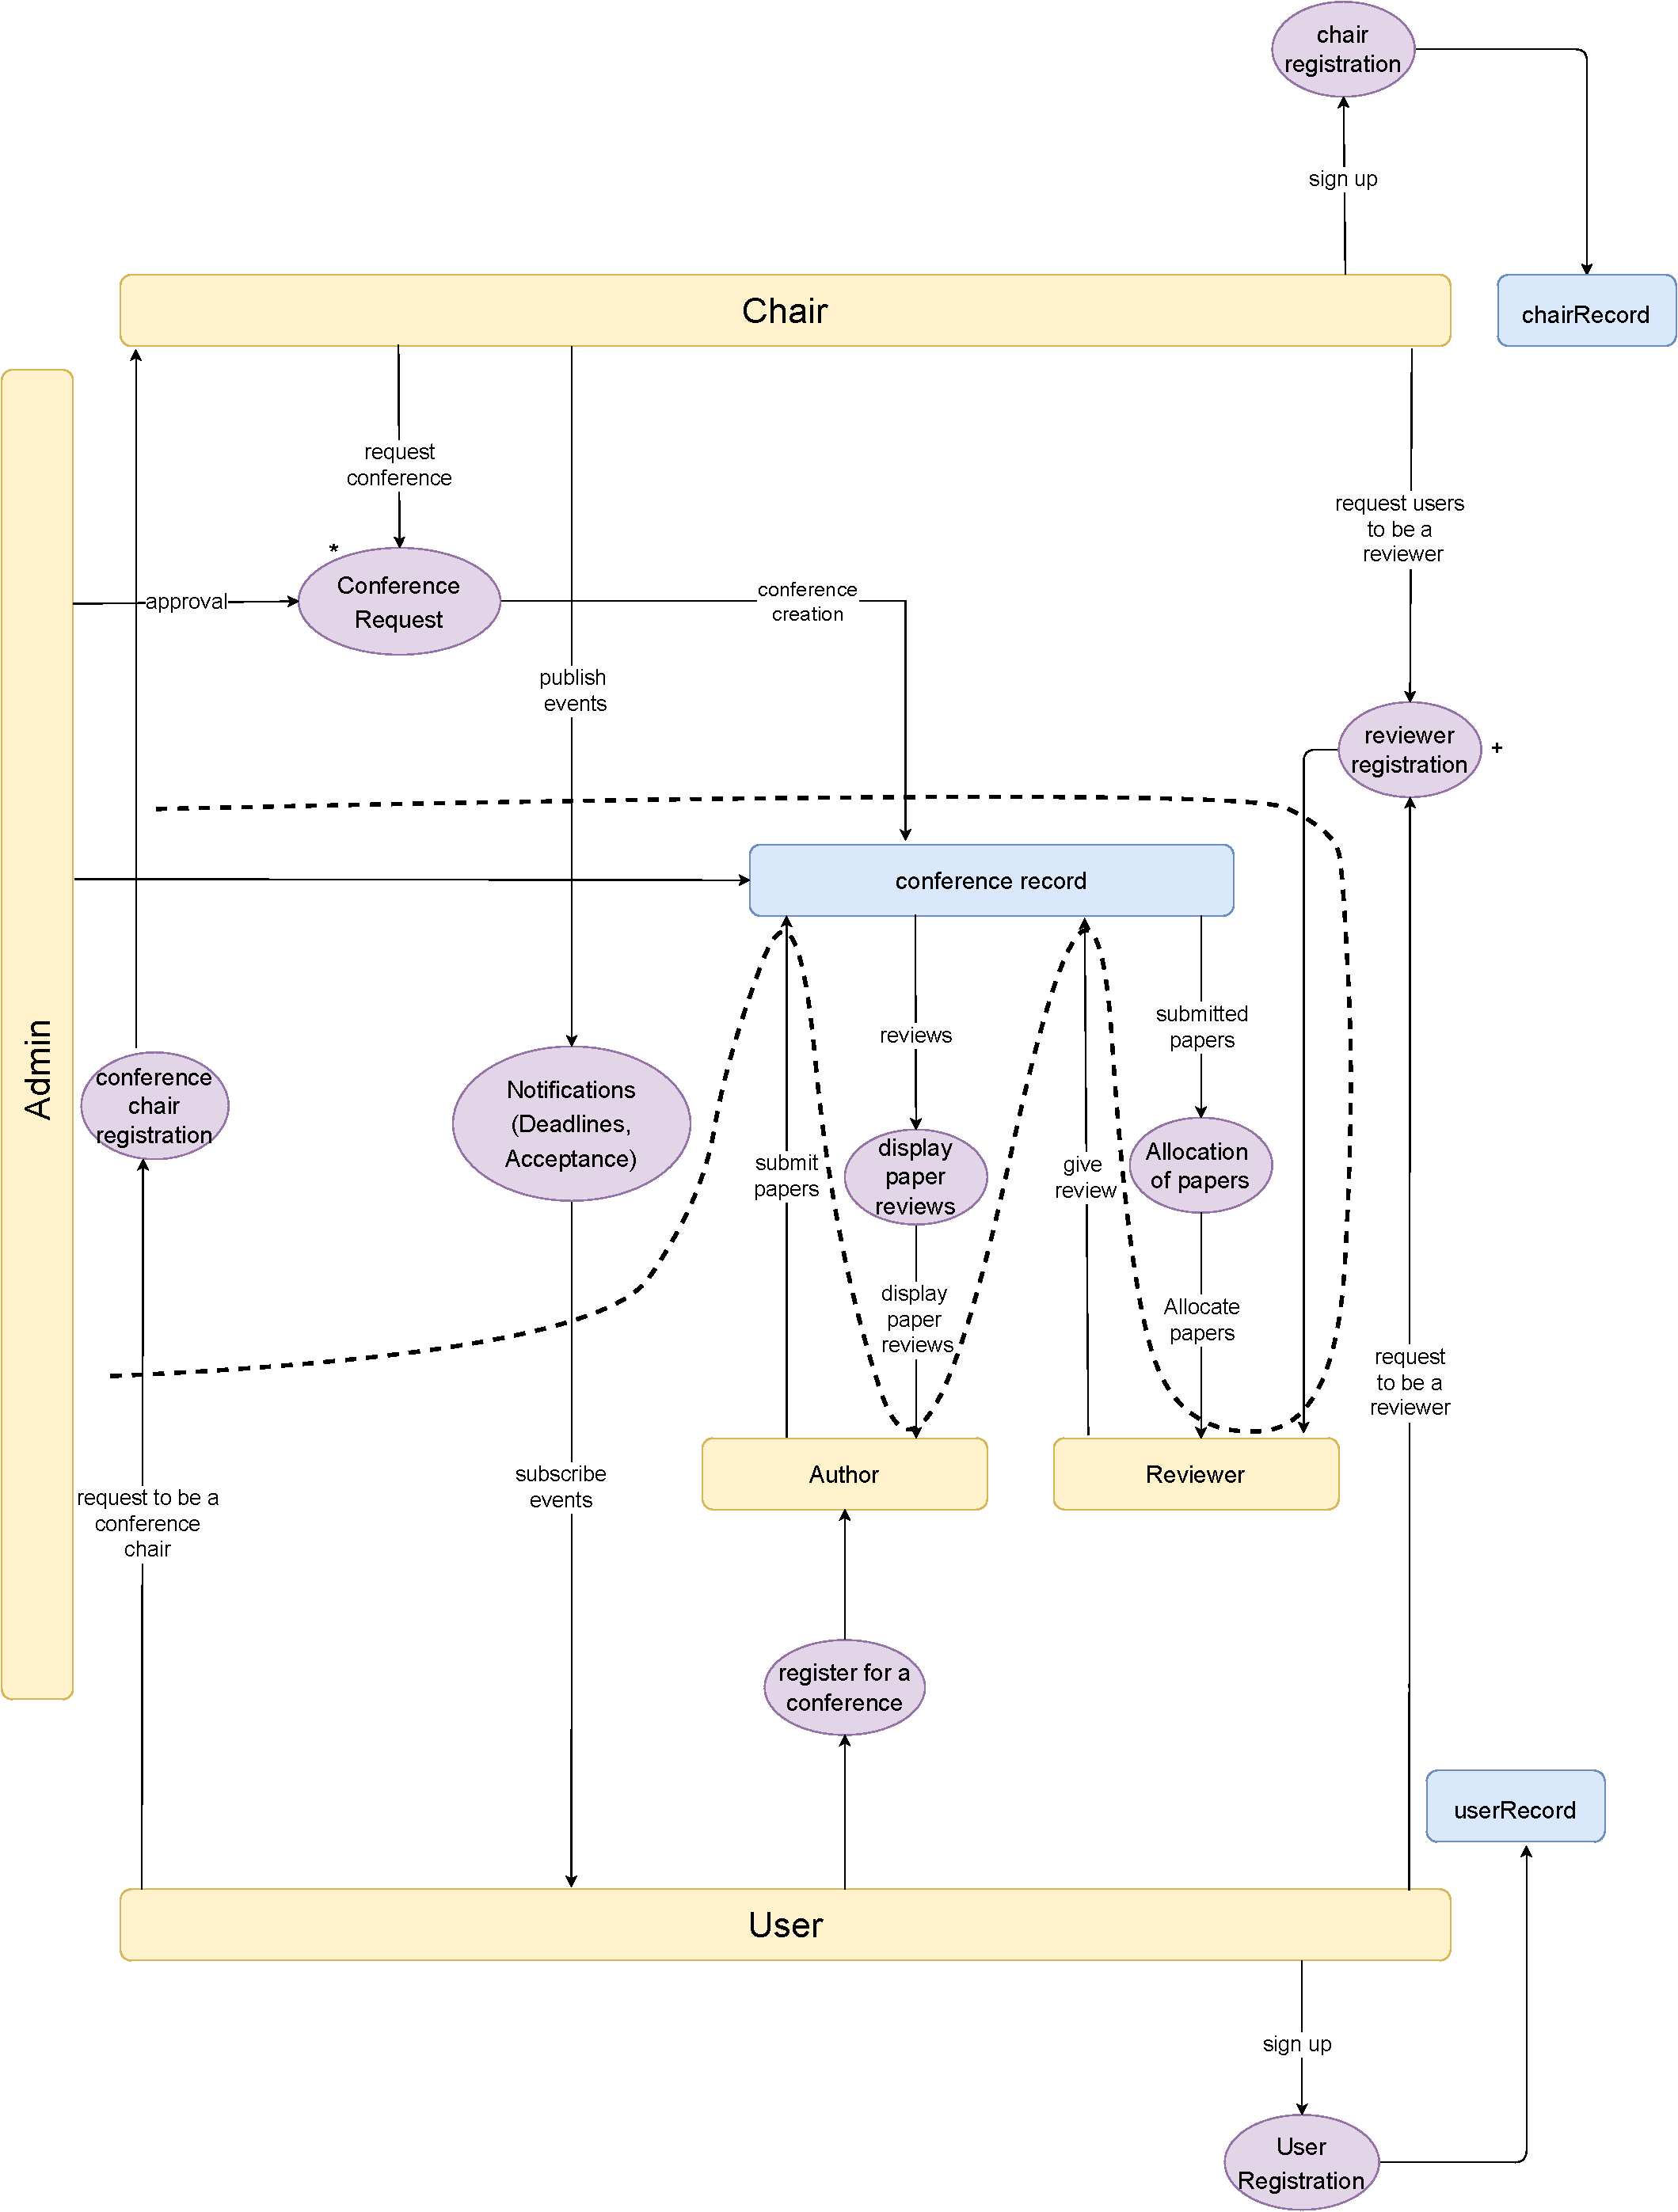
\includegraphics[keepaspectratio,height=16cm]{SRA-Images/DFD-final.pdf}
 \caption{Data Flow Diagram - Final}
 \addcontentsline{toc}{section}{Final DFD}
\end{figure}
\textbf{Improvements}
\begin{itemize}
    \item We inherited Authors and Reviewers from the users entity.
    \item An API is added for displaying reviews after the deadline to the authors and reviewers.
    \item Information regarding registration of chair to the conference portal is added.
    \item \textbf{Man-Machine Boundary}: Previous DFDs did not show any distinction between
automated and manual processes.
\item The conference records where all the details about the conference like details of papers and their respective authors are now managed by admin.

\end{itemize}
\end{enumerate}

    

\end{document}